\documentclass[landscape]{article}
\usepackage[landscape,margin=0.7in]{geometry}
\usepackage{pgfplots}
\usepackage{tikz}
\usepackage{xcolor}
\pgfplotsset{compat=1.18}

\begin{document}
\pagestyle{empty}

\begin{figure}
    \centering
    \begin{tikzpicture}
        \begin{axis}[
            title={\LARGE Boarding Strategy Comparison Summary},
            xlabel={Boarding Strategy},
            ylabel={Average Boarding Time (minutes)},
            symbolic x coords={Random, Back-to-Front, Outside-In, Hybrid},
            xtick=data,
            ybar,
            ymin=0,
            ymax=25,
            bar width=30pt,
            nodes near coords,
            nodes near coords align={vertical},
            width=0.85\textwidth,
            height=0.4\textheight,
            enlarge x limits=0.15,
            legend pos=north east,
            colormap/hot,
            axis lines=left,
            ymajorgrids=true,
            grid style=dashed
        ]
            
            \addplot[fill=red!70!black] coordinates {
                (Random, 18.7)
            };
            
            \addplot[fill=orange!70!black] coordinates {
                (Back-to-Front, 11.2)
            };
            
            \addplot[fill=green!70!black] coordinates {
                (Outside-In, 7.5)
            };
            
            \addplot[fill=blue!70!black] coordinates {
                (Hybrid, 10.0)
            };
            
            % Add improvement percentages
            \node[above, font=\small] at (axis cs:Hybrid,10.0) {-46.5\% vs Random};
            \node[above, yshift=1.5em, font=\small] at (axis cs:Hybrid,10.0) {-10.7\% vs Back-to-Front};
            \node[above, yshift=3em, font=\small] at (axis cs:Hybrid,10.0) {+33.3\% vs Outside-In};
        \end{axis}
    \end{tikzpicture}
\end{figure}

\begin{figure}
    \centering
    \begin{tikzpicture}
        \begin{axis}[
            title={\Large Boarding Time Ranges by Strategy},
            xlabel={Boarding Strategy},
            ylabel={Boarding Time (minutes)},
            symbolic x coords={Random, Back-to-Front, Outside-In, Hybrid},
            xtick=data,
            boxplot/draw direction=y,
            boxplot/box extend=0.5,
            width=0.8\textwidth,
            height=0.4\textheight,
            ymajorgrids=true,
            grid style=dashed
        ]
            \addplot+[
                boxplot prepared={
                    median=18.7,
                    upper quartile=20.5,
                    lower quartile=17.0,
                    upper whisker=21.9,
                    lower whisker=15.3
                },
                fill=red!60
            ] coordinates {};
            
            \addplot+[
                boxplot prepared={
                    median=11.2,
                    upper quartile=17.5,
                    lower quartile=5.0,
                    upper whisker=21.9,
                    lower whisker=1.9
                },
                fill=orange!60
            ] coordinates {};
            
            \addplot+[
                boxplot prepared={
                    median=7.5,
                    upper quartile=12.0,
                    lower quartile=3.0,
                    upper whisker=12.8,
                    lower whisker=2.0
                },
                fill=green!60
            ] coordinates {};
            
            \addplot+[
                boxplot prepared={
                    median=10.0,
                    upper quartile=15.0,
                    lower quartile=5.0,
                    upper whisker=18.7,
                    lower whisker=1.6
                },
                fill=blue!60
            ] coordinates {};
        \end{axis}
    \end{tikzpicture}
\end{figure}

\begin{figure}
    \centering
    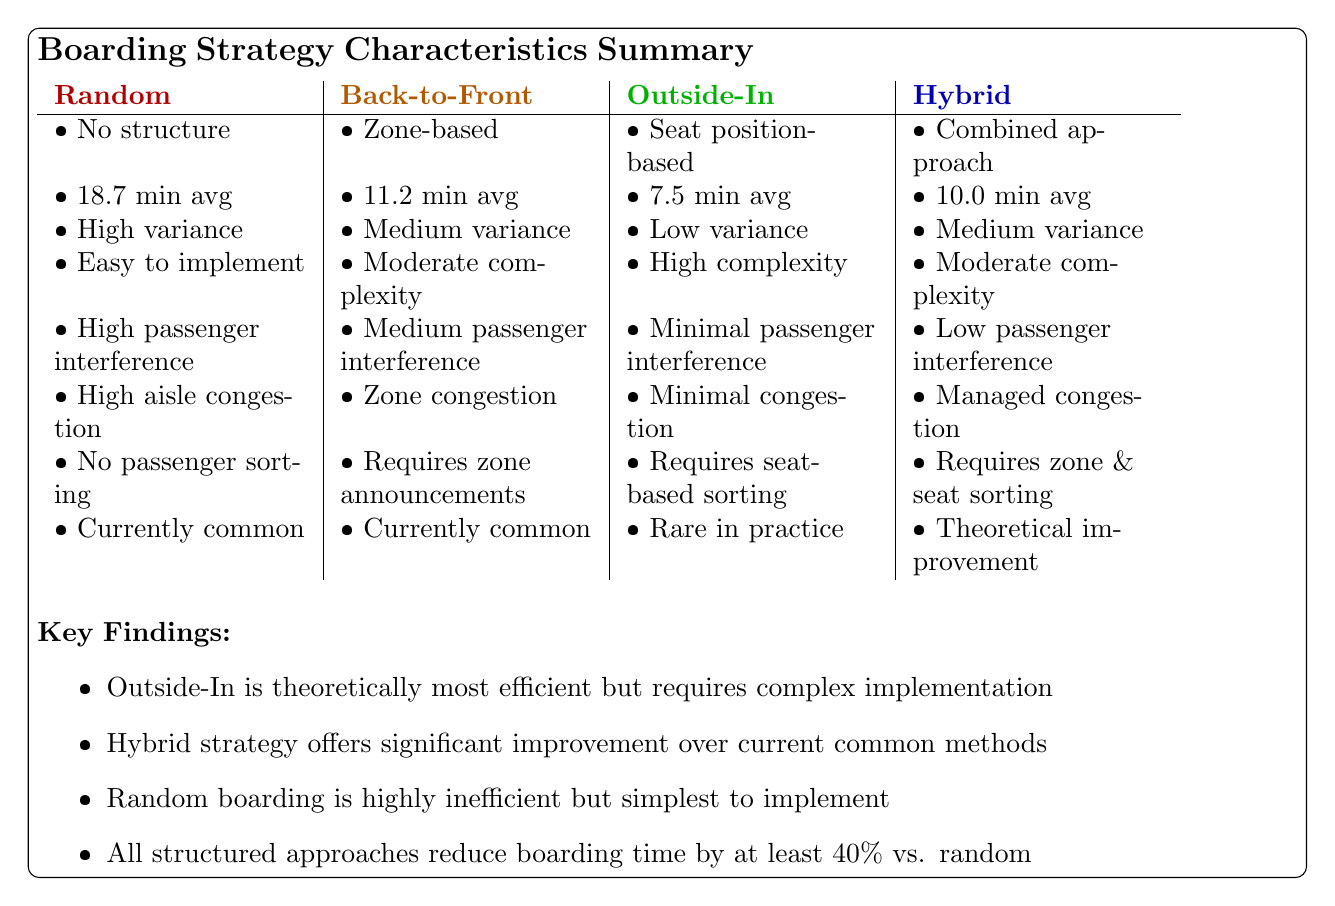
\begin{tikzpicture}
        \node[draw, align=left, anchor=center, text width=16cm, rounded corners] at (0,0) {
            \large\bfseries Boarding Strategy Characteristics Summary\\[0.3em]
            \normalfont\normalsize
            \begin{tabular}{p{3.2cm}|p{3.2cm}|p{3.2cm}|p{3.2cm}}
                \textbf{\textcolor{red!70!black}{Random}} & \textbf{\textcolor{orange!70!black}{Back-to-Front}} & \textbf{\textcolor{green!70!black}{Outside-In}} & \textbf{\textcolor{blue!70!black}{Hybrid}} \\
                \hline
                • No structure & • Zone-based & • Seat position-based & • Combined approach \\
                • 18.7 min avg & • 11.2 min avg & • 7.5 min avg & • 10.0 min avg \\
                • High variance & • Medium variance & • Low variance & • Medium variance \\
                • Easy to implement & • Moderate complexity & • High complexity & • Moderate complexity \\
                • High passenger interference & • Medium passenger interference & • Minimal passenger interference & • Low passenger interference \\
                • High aisle congestion & • Zone congestion & • Minimal congestion & • Managed congestion \\
                • No passenger sorting & • Requires zone announcements & • Requires seat-based sorting & • Requires zone \& seat sorting \\
                • Currently common & • Currently common & • Rare in practice & • Theoretical improvement \\
            \end{tabular}
            
            \vspace{0.5cm}
            \textbf{Key Findings:}
            \begin{itemize}
                \item Outside-In is theoretically most efficient but requires complex implementation
                \item Hybrid strategy offers significant improvement over current common methods
                \item Random boarding is highly inefficient but simplest to implement
                \item All structured approaches reduce boarding time by at least 40\% vs. random
            \end{itemize}
        };
    \end{tikzpicture}
\end{figure}

\end{document}